\section{Lanchesters Modelle}

\begin{karte}{Situation}
    2 Armeen: \(x,y\) im Kampf, 2 Arten von Verlusten: 
    \begin{enumerate}
        \item Operationsverlust: Verlust ohne Kämpfe (Krankheiten, Unfälle, \ldots) (wird vernachlässigt)
        \item Verluste durch Kämpfe: Ist \(x\) eine konventionelle Armee, so kann 
        jeder Gegner \(y\) einen Verlust in \(x\) erzielen.\\
        Annahme: proportional zu \(y\), d. h. \(\alpha y(t)\)
        Ist \(x\) eine Guerilla, handelt im Verborgenen, so werden sie von \(y\) 
        nicht gesehen \(\leadsto\) Verlustrate von \(x\) ist proportional zu \(x\) und \(y\)
        \(\leadsto \) Verlustrate ist \(c x(t) y(t)\).
    \end{enumerate}
\end{karte}

\begin{karte}{Modelle}
    Konventioneller Kampf: 
    \[ \begin{cases}
        \frac{dx}{dt} = -ay + f(t) \\
        \frac{dy}{dt} = -bx + g(t)
    \end{cases} \]
    Konventioneller Guerilla Kampf: 
    \[ \begin{cases}
        \frac{dx}{dt} = -cxy + f(t) \\
        \frac{dy}{dt} = -dx + g(t)
    \end{cases} \]
    Konventioneller Kampf ist linear und kann explizit gelöst werden, 
    Guerilla Kampf ist nicht linear und kann i. A. nur numerisch gelöst werden.\\
    Annahme: es gibt keine Verstärkung, also \(f = g \equiv 0\).
\end{karte}

\begin{karte}{Wurzelgesetz 1}
    Wenn keine Verstärkung kommt, so folgt 
    \[ \frac{dy}{dx} = \frac{\frac{dy}{dt}}{\frac{dx}{dt}} = \frac{bx}{ay} 
    \Leftrightarrow ay \frac{dy}{dx} = bx \]
    und durch Integrieren folgt 
    \[ ay^2 - bx^2 = ay_0^2 - bx_0^2 = K \in \R \]
    Diese Gleichung beschreibt Hyperbeln in der \(x\)-\(y\)-Ebene.
    \begin{center}
        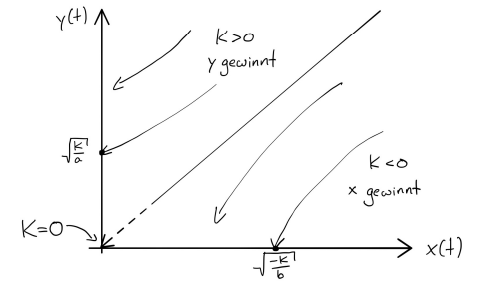
\includegraphics[width=0.4\textwidth]{img/wurzelgesetz.png}
    \end{center}
\end{karte}

\begin{karte}{Wurzelgesetz 2}
    Ist \(K>0\), so folgt \(\limes{t} x(t) = 0\) und \( \limes{t} = \sqrt{K/a}\) 
    und umgekehrt. \(K\) kann positiv gemacht werdne, indem man 
    \begin{enumerate}
        \item \(a\) erhöht.
        \item \(y_0\) erhöht.
    \end{enumerate}
    Verdoppelt man \(a\) (bessere Waffen), so wird \(ay_0^2\) verdoppelt. 
    Verdoppelt man \(y_0\), so wird \(ay_0^2\) vervierfacht.
\end{karte}

\begin{karte}{Konventionell-Guerilla}
    Die Orbits sind Lösungen 
    \[ \frac{dy}{dx} = \frac{\frac{dy}{dt}}{\frac{dx}{dt}} = \frac{dx}{cxy} 
    = \frac{d}{cy} \]
    Integrieren liefert 
    \[ cy^2 - 2dx = cy_0^2 - 2dx_0 = M\in \R \]
    Dies definiert Parabeln in der \(x\)-\(y\)-Ebene: 
    \begin{center}
        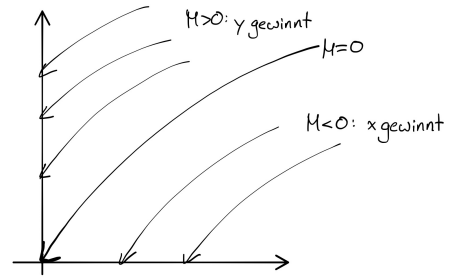
\includegraphics[width=0.4\textwidth]{img/parabeln-guerilla.png}
    \end{center}
\end{karte}